\documentclass[tikz,convert={outext=.png}]{standalone}
\begin{document}
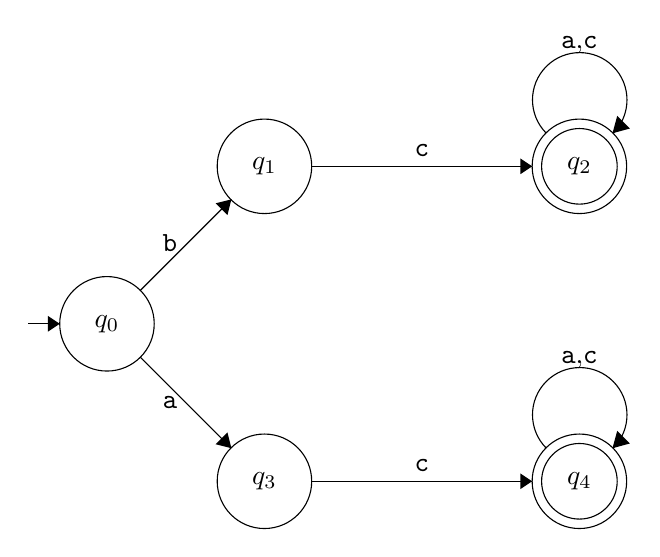
\begin{tikzpicture}[scale=0.2]
\draw [black] (-5,0) -- (-3,0);
\fill [black] (-3,0) -- (-3.75,-.5) -- (-3.75,.5);
\draw [black] (0,0) circle (3);
\draw (0,0) node {$q_0$};

\draw [black] (2.1, 2.1) -- (7.9,7.9);
\fill [black] (6.9,7.65) -- (7.9,7.9) -- (7.65,6.9);
\draw (4,4) node [above] {{\tt b}};
\draw [black] (10,10) circle (3);
\draw (10,10) node {$q_1$};

\draw [black] (2.1, -2.1) -- (7.9,-7.9);
\fill [black] (6.9,-7.65) -- (7.9,-7.9) -- (7.65,-6.9);
\draw (4,-4) node [below] {{\tt a}};
\draw [black] (10,-10) circle (3);
\draw (10,-10) node {$q_3$};

\draw [black] (13,10) -- (27,10);
\fill [black] (27,10) -- (26.25,10.5) -- (26.25,9.5);
\draw (20,10) node [above] {{\tt c}};
\draw [black] (30,10) circle (3);
\draw [black] (30,10) circle (2.4);
\draw (30,10) node {$q_2$};
\draw (27.9,12.1) arc (225:-45:3);
\fill [black] (32.1,12.1) -- (32.4,13.2) -- (33.2,12.4);
\draw (30,16.5) node [above] {{\tt a},{\tt c}};

\draw [black] (13,-10) -- (27,-10);
\fill [black] (27,-10) -- (26.25,-10.5) -- (26.25,-9.5);
\draw (20,-10) node [above] {{\tt c}};
\draw [black] (30,-10) circle (3);
\draw [black] (30,-10) circle (2.4);
\draw (30,-10) node {$q_4$};
\draw (27.9,-7.9) arc (225:-45:3);
\fill [black] (32.1,-7.9) -- (32.4,-6.8) -- (33.2,-7.6);
\draw (30,-3.5) node [above] {{\tt a},{\tt c}};
\end{tikzpicture}
\end{document}
